\chapter{Simultaneous viewing of images and surfaces}

The simultaneous viewing of images and surfaces can be activated clicking the \textbf{left} mouse button on the shortcut located in the lower right corner of the InVesalius screen. See figure~ \ref{fig:slice_plane_original}.

\begin{figure}[!htb]
\centering

\includegraphics[scale=0.6]{slice_plane_original}
\caption{Shortcut for simultaneous viewing}
\label{fig:slice_plane_original}
\end{figure}

This feature allows enable or disable the display of images in different orientations (or plans) within the same display window of the 3D surface. To do this, simply check or uncheck the corresponding option in the menu shown in figure~\ref{fig:view_2d_3d_1}.

\begin{figure}[!htb]
\centering
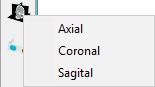
\includegraphics[scale=0.6]{view_2d_3d_1_en.png}
\caption{Selection of the guidelines (plans) to display}
\label{fig:view_2d_3d_1}
\end{figure}

It is worth noting when the particular orientation is selected, a check is presented in the corresponding option. This is illustrated in figure~\ref{fig:view_2d_3d_2}.

\begin{figure}[!htb]
\centering
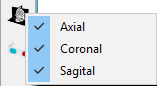
\includegraphics[scale=0.6]{view_2d_3d_2_en.png}
\caption{Selected Guidelines for display}
\label{fig:view_2d_3d_2}
\end{figure}

\newpage

If the surface is already displayed, the plans of the guidelines will be presented as shown in figure~\ref{fig:only_2d_planes}. Otherwise, only the plans will be displayed

\begin{figure}[!htb]
\centering
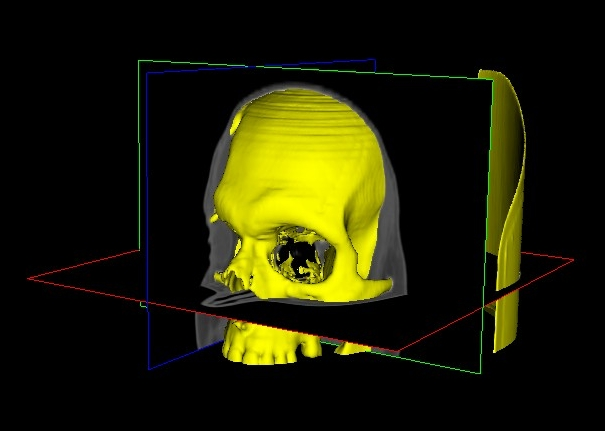
\includegraphics[scale=0.5]{3d_planes}
\caption{Surface and plans displayed simultaneously}
\label{fig:3d_planes}
\end{figure}

\begin{figure}[!htb]
\centering
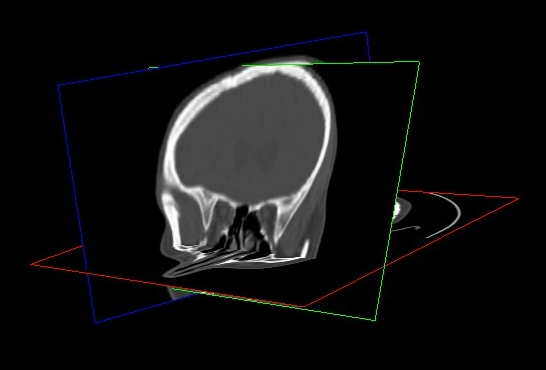
\includegraphics[scale=0.55]{only_2d_planes}
\caption{Flat display (no surface)}
\label{fig:only_2d_planes}
\end{figure}

\newpage

To view the display of a plan, just uncheck the corresponding option in the menu (figure~\ref{fig:view_2d_3d_2})